30. \begin{figure}[ht!]
\center{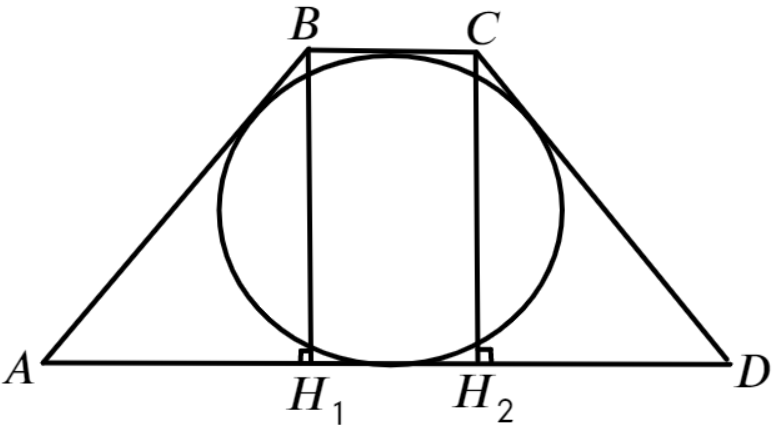
\includegraphics[scale=0.35]{g8-29.png}}
\end{figure}\\
Так как трапеция является описанным четырёхугольником, суммы его противоположных сторон равны. Так как она равнобедренная, $2AB=2CD=BC+AD=32+50=82,\ AB=CD=41$см. Опустим две высоты $BH_1$ и $CH_2,$ тогда $H_1H_2=BC=32$см, $AH_1=DH_2=(50-32):2=9$см. По теореме Пифагора $BH_1=\sqrt{41^2-9^2}=40$см. Тогда $R=BH_1:2=40:2=20$см.
ewpage
oindent
